\paragraph{}{
	L'Unité Arithmétique et Logique, abrégé UAL, permet de faire des calculs
	basiques (additions, divisions, décallages de bits, etc.). Elle travaille
	sur 
}

\begin{figure}
	\centering
	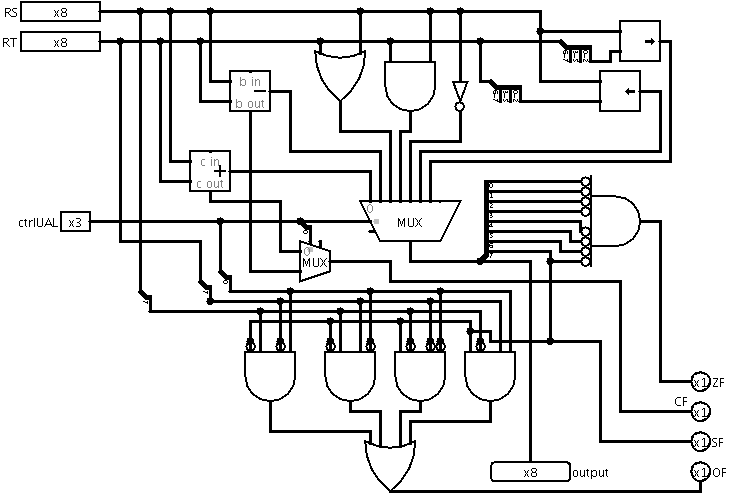
\includegraphics[scale=0.5,origin=c]{circuits/UAL.png}
	\label{ual_circ}
	\caption{Sch\'{e}ma \'{e}lectronique de l'Unit\'{e} Arithm\'{e}tique et Logique}
\end{figure}